\chapter{
%Modeling Animal space-usage with 
%Detection Models based on Ecological Distance
Ecological Distance Models in Spatial Capture-Recapture
}
\markboth{Chapter XXX}{}
\label{chapt.implicit}


\vspace{.3in}


Previously we have only considered stationary and symmetric models for
detection probability. While these will often be sufficient for
practical purposes, especially in small data sets, there will
sometimes be interest in developing more complex models of the
detection process as it relates to space usage of individuals.  

These models are simple because they are based on
Euclidean distance -- which are convenient because we know this
distance precisely conditional on individual activity center ${\bf  s}$.
However, animals may not
judge distance in terms of euclidean distance but, rather, according
to local habitat conditions and so forth. 

In this section we develop models for detection probability based on
alternative distance metrics that account for ecological
considerations -- what we will call ``ecological distance''. In
particular, we adopt a cost-weighted distance metric which is an idea
in widespread use in 
landscape ecology for modeling connectivity, movement and gene flow
\citep{adriaensen_etal:2003,manel_etal:2003,mcrae_etal:2008}. In the context of SCR
models we can use this as the basis for computing the distance
bwetween traps and individuals activity centers. In this way we can
explicitly accommodate some landscape structure and ideas related to how animals
use space in SCR models. 

Moreoever, we can estimate parameters of thos distance
metrics..... for the first time in the history of mankind, we do that
here. 


\section{Cost Distance}

We use a cost-weighted distance metric in the package \mbox{\tt
  gdistance} \index{R package!gdistance} which computes the distance between points by
accumulating pixel-specific costs assigned by the user (but we
consider estimating these in Sec. XYZ). The idea is widely used in
landscape ecology for modeling connectivity, movement and gene flow
\citep{adriaensen_etal:2003,mcrae_etal:2008}.
The basic idea is that distance bewtween $x_{i}$ and $x_{j}$ is
\[
 wd_{ij} =  w_{ij} ....\mbox{formula for this?}
\]
where .... and so on....XXX XYZ.
To be consistent with the functioning of \mbox{\tt costDistance} the
incremental cost is assessed for {\it leaving} a pixel, not
arriving. As a consequence, the terminal value is not counted. 
In addition to \mbox{\tt gdistance} we use functions from a number of
other {\bf R} packages including \mbox{\tt rgeos}, \mbox{\tt
  shapefiles} and \mbox{\tt raster}.

As an example of the cost-weighted distance calculation consider the
following landscape comprised of 16 pixels with unit spacing 
identified as follows, along
with the pixel-specific cost:
\begin{verbatim}
  pixel ID                 Cost
  1  2  3  4          100   1   1  1
  5  6  7  8          100 100   1  1
  9 10 11 12          100 100 100  1
 13 14 15 16          100 100   1  1 
\end{verbatim}
Then we assign low cost of 1 to ``good habitat'' pixels (or pixels we
think of as ``highly connected'' by virtue of being in good habitat)
and, conversely, we assign high cost (100) to ``bad habitat''. So the
shortest cost-weighted distance between pixels 2 and 3 in this example
is just 1 unit, the shortest cost-distance between pixels 2 and 7 is
sqrt(2) units, the shortest distance between pixels 13 and 14 is 100
units, while the shortest cost-distance between 13 and 15 is 100. A
tough one is: what is the shortest distance between 10 and 16? A guy at pixel
10 can move diagonal and pay sqrt(2)*1 + 1 total.
An alternative pixel labeling scheme arising as if you were applying
the vec operation to the matrix ``as you look at it''. This produces
labels that are a transpose of those given previously, so the id's are
as follows:
\begin{verbatim}
 1 5  9 13
 2 6 10 14
 3 7 11 15
 4 8 12 16
\end{verbatim}
In this case we have to transpose or rotate something along the way. 
Be careful. This matters in the way you stick the ``cost'' data into
the elements of the raster.
In the following example we fill the cost
matrix using the default \mbox{\tt byrow=FALSE} standard in {\bf
  R}, but here we use cost values of 1-16 so that we can produce an
image of the resulting costs to visualize their ordering in the raster:
\begin{verbatim}
r<-raster(nrows=4,ncols=4)
projection(r)<- "+proj=utm +zone=12 +datum=WGS84"
extent(r)<-c(.5,4.5,.5,4.5)
values(r)<-matrix(1:16,4,4,byrow=FALSE)
par(mfrow=c(1,1))
plot(r)
\end{verbatim}
The raster, in image form, is shown in Fig. \ref{ecoldist.fig.raster}.

\begin{figure}
\begin{center}
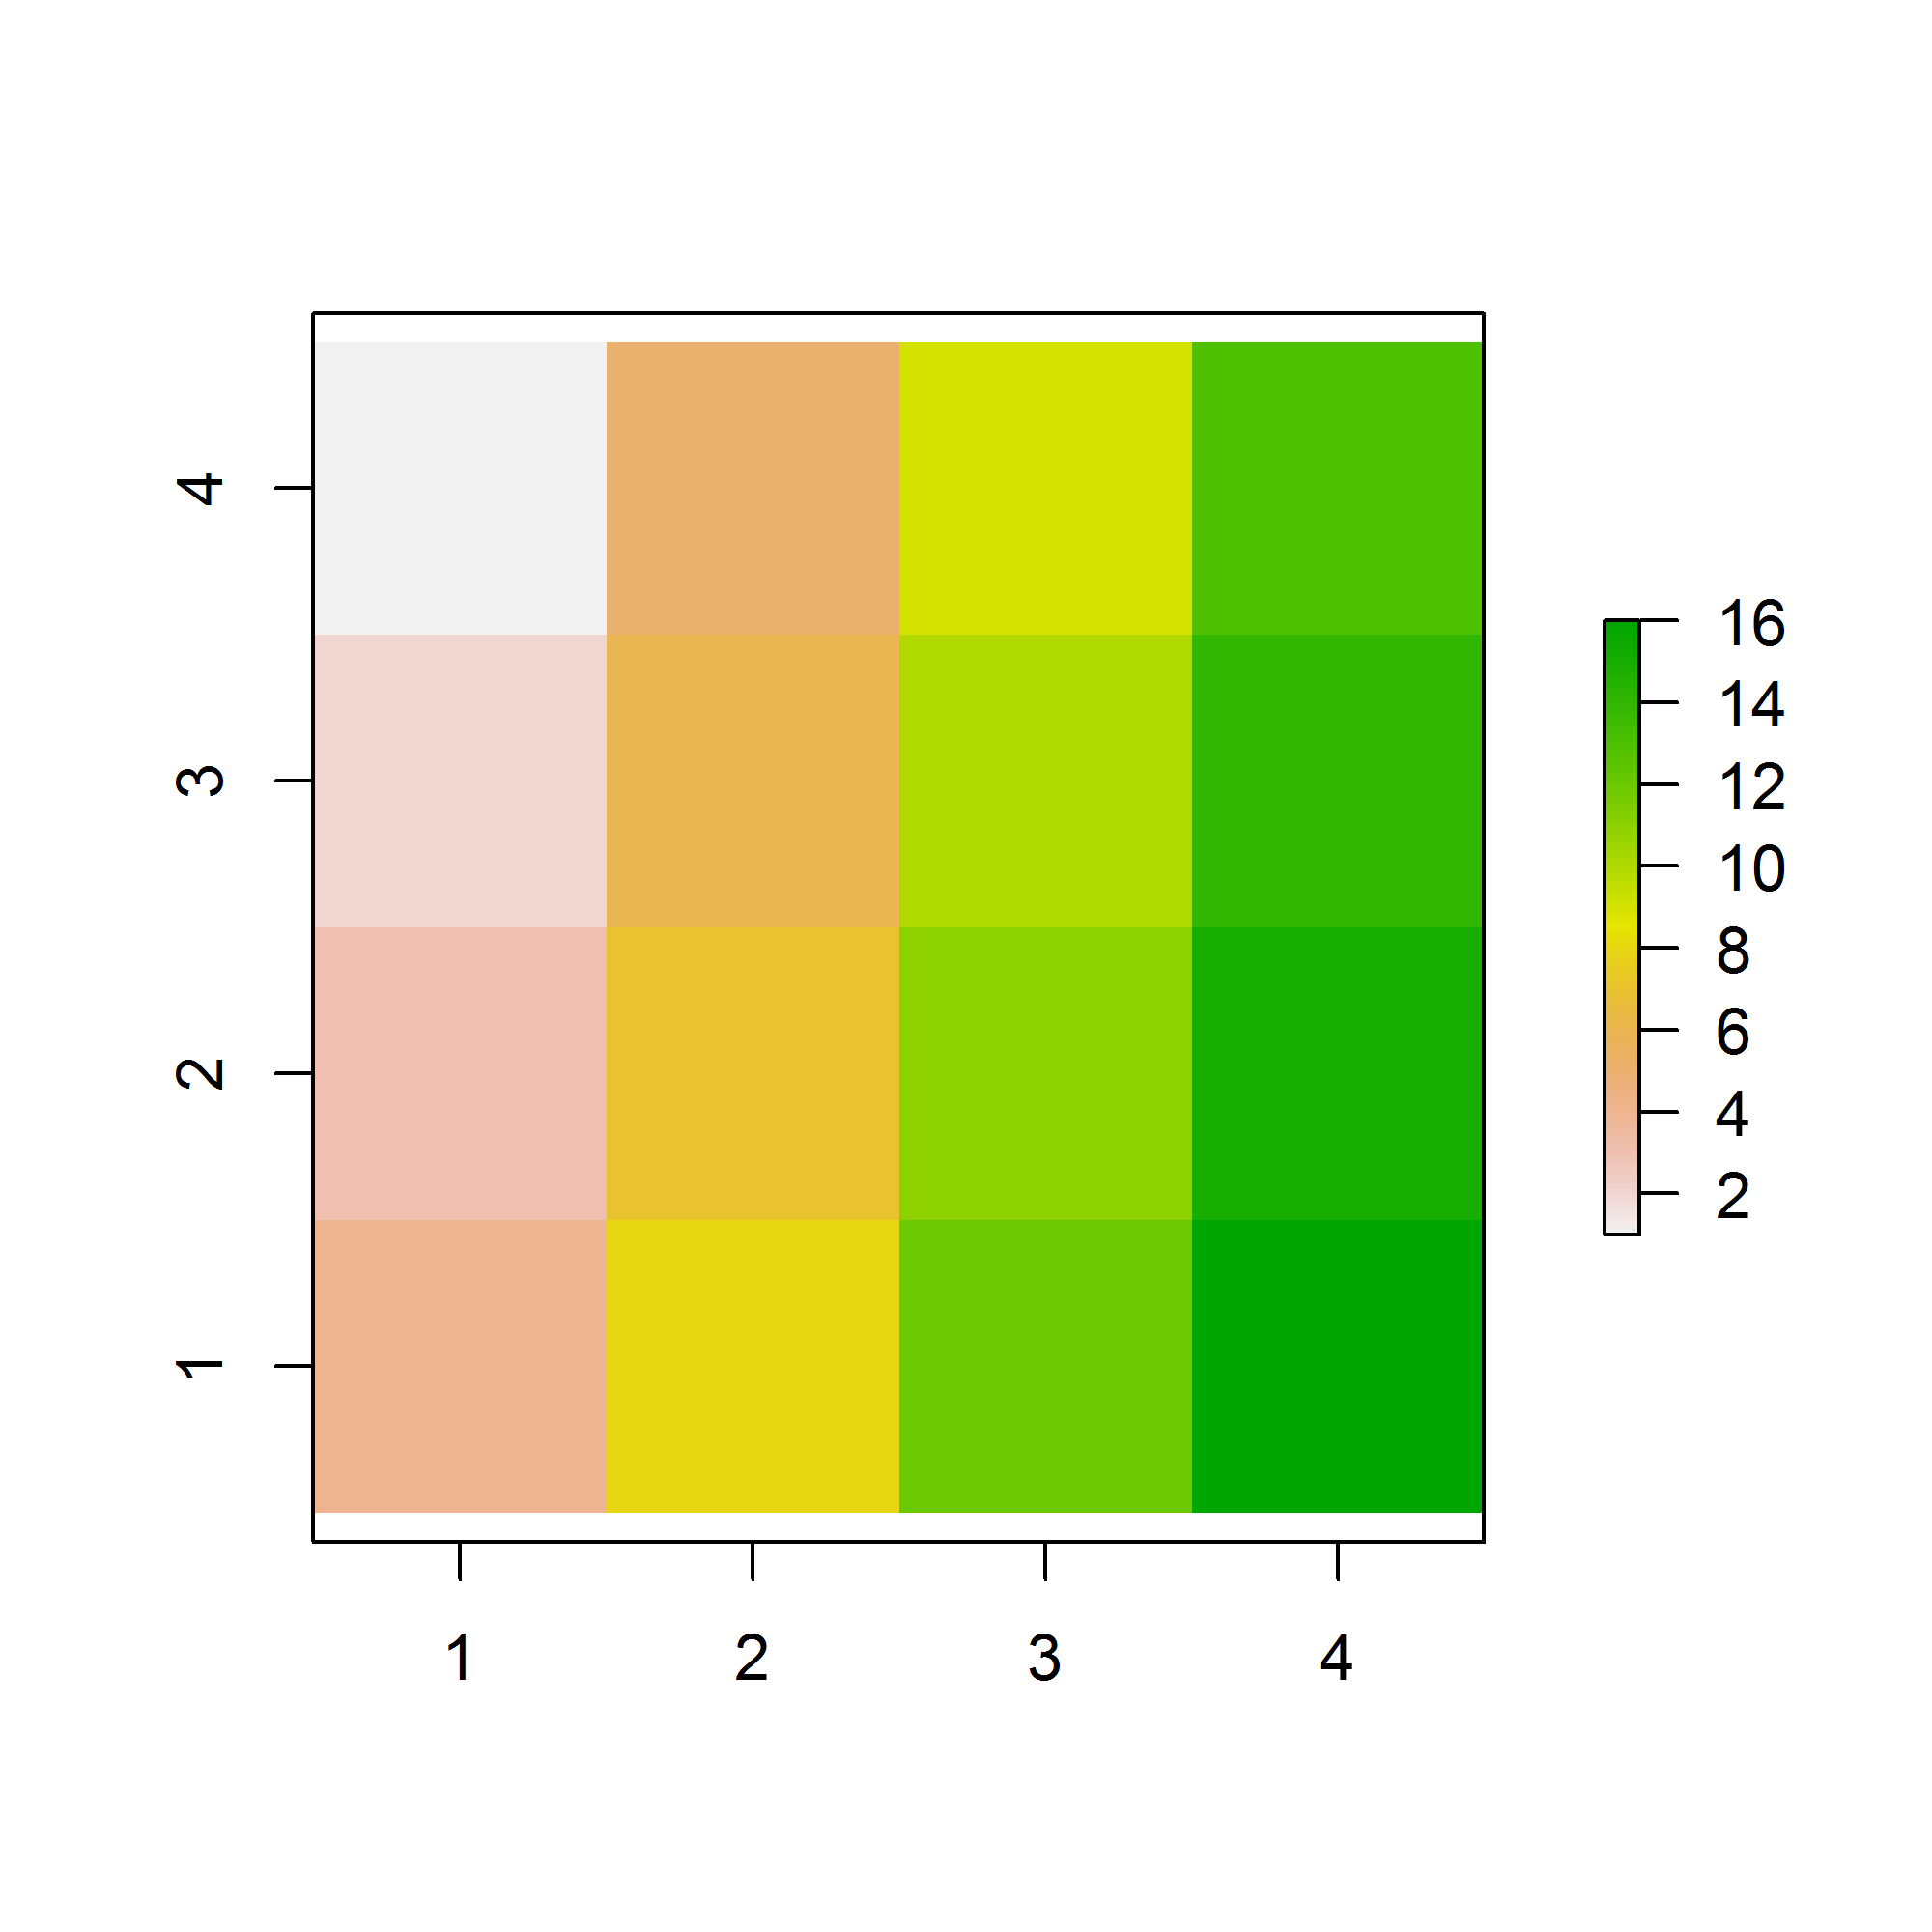
\includegraphics[height=3.25in,width=3.25in]{Ch10/figs/raster}
\end{center}
\caption{a 16 pt raster}
\label{ecoldist.fig.raster}
\end{figure}

Then we use the functions \mbox{\tt transition}, \mbox{\tt
  geoCorrection} (which doesn't really do anything but reformat the
data somehow) and \mbox{\tt costDistance} to compute the distance
matrix. They operate on this inverse-scale so we first take the element-by-element
inverse of the raster. Then we define a set of points,
the center points of each raster, to compute the cost-distance between
them all. The commands altogether are as follows:
\begin{verbatim}
r<-1/r
tr1<-transition(r,transitionFunction=max,directions=8)
tr1CorrC<-geoCorrection(tr1,type="c",multpl=FALSE,scl=FALSE)
pts<-cbind( sort(rep(1:4,4)),rep(4:1,4))
costs1<-costDistance(tr1CorrC,pts)
outD<-as.matrix(costs1)
\end{verbatim}
Now we can look at the result and see if it makes sense to us. Here we
print the first 4 columns of this distance matrix and illustration a
couple of examples of calculating the minimum cost-weighted distance
between points:
\small{
\begin{verbatim}
     1    2    3    4   
1   0.0  1.0  3.0  6.0  
2   1.0  0.0  2.0  5.0  
3   3.0  2.0  0.0  3.0  
4   6.0  5.0  3.0  0.0  
5   1.0  2.0  4.0  7.0  
6   1.4  2.0  4.0  7.0  
7   3.8  2.8  3.0  5.7  
8   7.2  6.2  4.2  4.0  
9   6.0  7.0  9.0 12.0  
10  7.4  8.0 10.0 13.0  
11  9.9  9.8 10.0 12.7 
12 13.7 12.7 12.2 12.0 
13 15.0 16.0 18.0 21.0 
14 17.4 18.0 20.0 23.0 
15 20.9 20.8 21.0 23.7 
16 25.5 24.7 24.2 24.0 
\end{verbatim}
}
Moving down the first (left-most, as you look at it) column of the
raster the cost-distance between pixel 1 and 2 is 1.0 which we know to
be right because the cost of leaving pixel 1 is tabulated, and that is
the value 1.0.  To get from pixel 1 to pixel 3 we have to leave both
pixels 1 and 2, for a total cost of $1+2 = 3$ which is the result
given above.  To see that the shortest cost-weighted distance is not always the
shortest Euclidean distance, consider moving from pixel .....


\section{Examples of Computing Cost-Distance}

In this section we provide a series of examples that we think
represent how cost-weighted distance models will be used in real
problems. The basic framework for analysis is based on R packages XYZ
and functions XYZ to do basic operations involving polygons and point
files.

In particular, we will typically have a polygon coverage either in the
form of a GIS shapefile or a matrix of points or some other specific
format, and we want to put that polygon on a map and use the polygon
boundary in some way to generate pixel-specific costs. So we want to
see if points or raster pixels are in the polygon, or not, or how far
they are from the polygon boundary (cost might be related to distance)
and similar operations. In the following examples, we confront how to
do some of these operations in {\bf R}. 


\subsection{Illustration: Example Good vs. Bad habitat}

Here we analyze the cost-weighted distance for a landscape created to
mimic
a habitat corridor or park unit or some other block of
relatively homogeneous good-quality habitat for some species
(Fig. \ref{ecoldist.fig.corridor}).
It is surrounded by a suburban wasteland of McDonalds and Wal-Marts, much
less hospital habitat for most things. See
We describe the steps for creating this landscape shortly, so that the
reader can use a similar process to generate more relevant landscapes
for their own problems. 

In practice, we have a landscape with multiple polygons delineating
good or bad habitat or a forest preserve or corridors or
whatever. These exist maybe as shapefiles.
We have to create a raster, overly the polygon and assign values
depending on whether pixels are in good polygons or not.
You can do this in GIS but we do a version of this in R here. See
chapter 5.XYZ for an example of reading in the shapefile and doing it.

We provide 
 a function \mbox{\tt make.seg} which allows the user to make a specific
buffer given a trap region.  You can plot the region with a range or a
specific set of points and then click over it using these commands:
{\small 
\begin{verbatim}
make.seg<-function(npts){
l2<-locator(npts)
l2<-cbind(l2$x,l2$y)
l2<-round(l2,2)
tmp<-NULL
for(i in 1:nrow(l2)){
tmp<-paste(tmp,l2[i,1],l2[i,2])
if(i<nrow(l2))
tmp<-paste(tmp,",")
}
l2b<- paste("LINESTRING(",tmp,")")
l2<- readWKT(l2b)
return(l2)
}


plot(NULL,xlim=c(0,10),ylim=c(0,10))
l1<-make.seg(9)
plot(l1)
l2<-make.seg(5)
plot(l1)
lines(l2)
\end{verbatim}
}
We used this function to create a couple of line segments of class XXX
from package xyz XXXXXX  which can be loaded as 
follows\footnote{how to put this in the R package?}:
\begin{verbatim}
load("polygons.RData")
\end{verbatim}
This has 2 polygon files in it ......representing different segments
of this corridor or river system. We use the commands XYZ to join and
buffer the two segments and the resultt is that shown in fig. XYZ.

\begin{verbatim}
buffer<- 0.5
l1<-l1.old
l2<-l2.old
par(mfrow=c(1,1))
aa<-gUnion(l1,l2)
plot(gBuffer(aa,width=buffer),xlim=c(0,10),ylim=c(0,10))
pg<-gBuffer(aa,width=buffer)
pg.coords<- pg@polygons[[1]]@Polygons[[1]]@coords

xg<-seq(0,10,,30)
yg<-seq(10,0,,30)

delta<-mean(diff(xg))
pts<- cbind(sort(rep(xg,30)),rep(yg,30))
points(pts,pch=20)

in.pts<-point.in.polygon(pts[,1],pts[,2],pg.coords[,1],pg.coords[,2])
points(pts[in.pts==1,],pch=20,col="red")

\end{verbatim}

\begin{figure}
\begin{center}
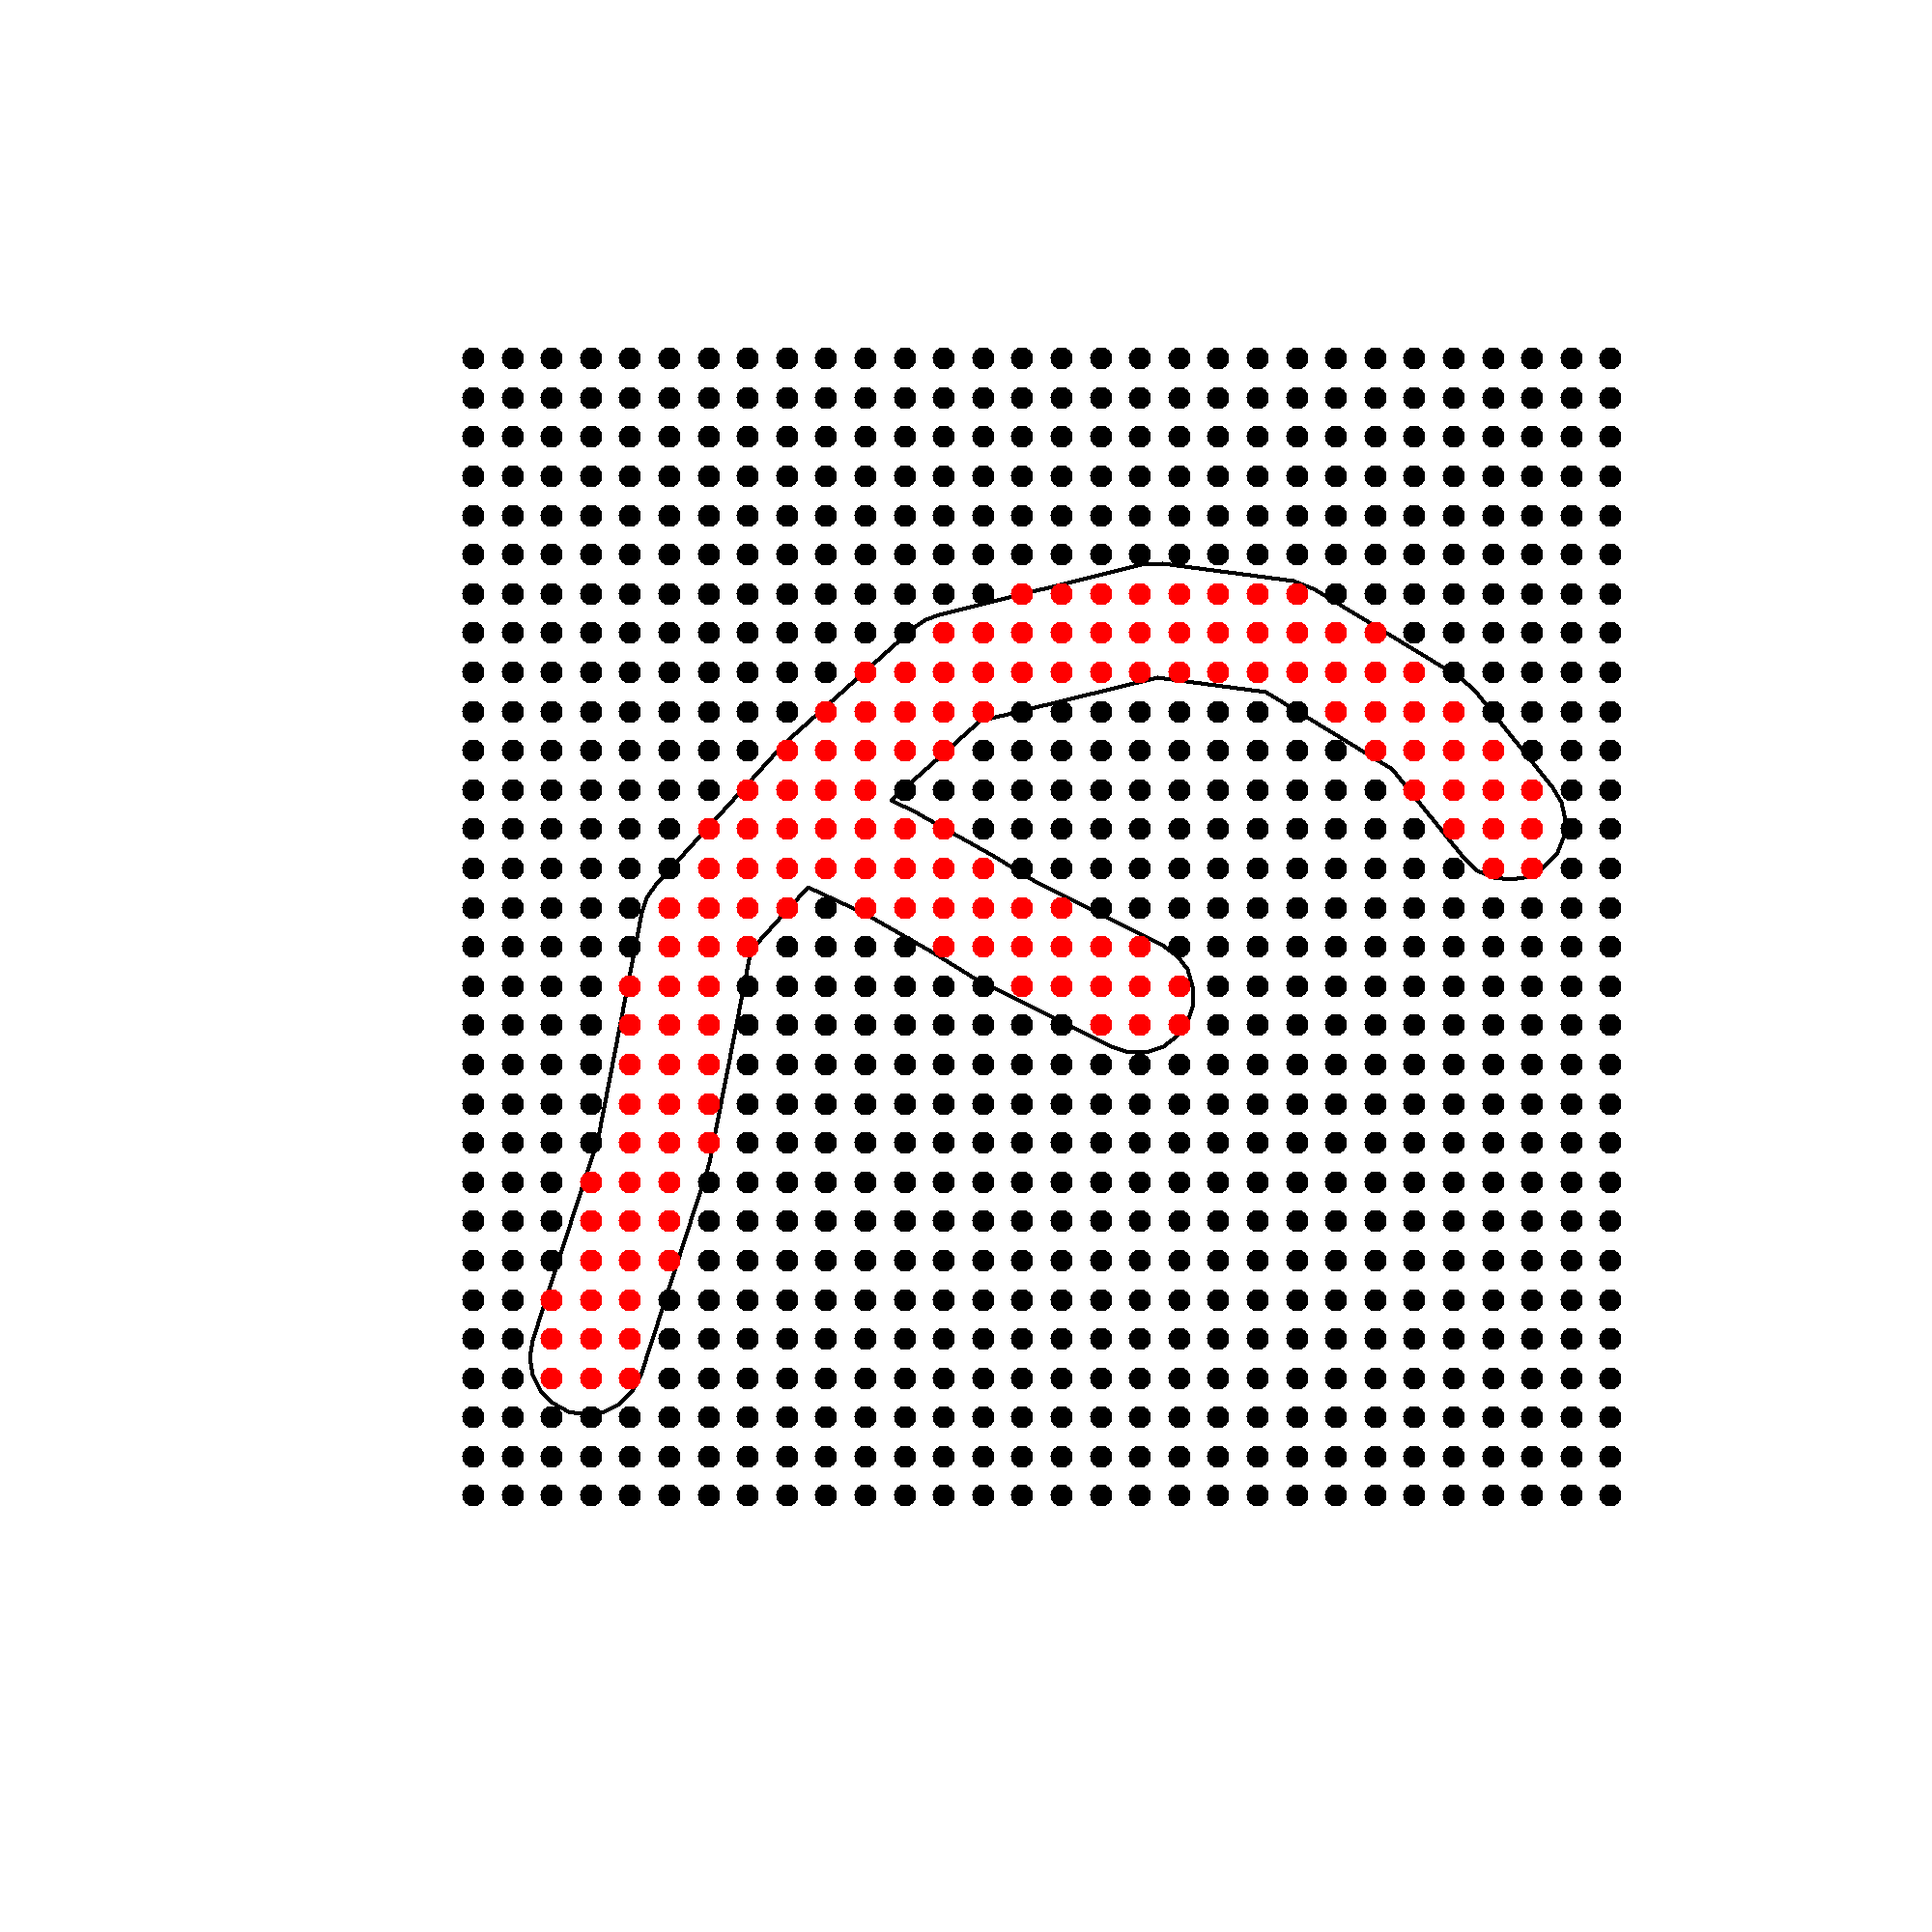
\includegraphics[height=3.25in,width=3.25in]{Ch10/figs/corridor}
\end{center}
\caption{a habitat corridor or preserve}
\label{ecoldist.fig.corridor}
\end{figure}


We focus on devising a SCR model for this corridor system and we
imagine that animals will tend to severely avoid leaving the buffered
habitat zone.

\subsection{Distance Weighting}

We consider a situation here in which we develop weights based on the
distance from some feature such as a highway or a river. 

\subsection{Hard Boundary}

\section{Ecological distance in SCR models}

Code for fitting the basic model  with minimum cost-distance {\it fixed}.



\section{Real example}


\section{Estimating Cost or Resistance Values}

\section{Bayesian Analysis}

Some of this stuff can be done easily enough in BUGS or we can code
our own. e.g., we only need the distance matrix computed ahead of time
and we can work on that with a discrete raster.  continuous space is
less easy because BUGS doesn't have a function for computing
ecological distance between any arbitrary points. 

As for estimating the parameters of the ecological distance function
-- this might at the present time be impossible in the BUGS
variants. However, we can use the functions described above to
implement our own MCMC algorithm following the developments of
Chapt. \ref{chapt.mcmc}.


\section{Summary and Outlook}

This shit is hot. We are the man. There is no limit to what we can do.


The effect of ignoring ecological distance e.g. if that is the true
data generating model would be useful to investigate for some specific
situations. obviously this will depend on the complexity of the
landscape being considered and the actual manner in which animals use
space, i.e., how they perceive distance. Since we can never know this,
any kind of sim study would be inherently arbitrary and so we didn't
pursue that here. [i guess i mean we never ever can observe actual
costs at the pixel level or even get directinfo about that because we
only observe the total distance traveled -- and that is only observed
imperfectly -- so getting direct info about cost seems difficult and
maybe not even possible. 
If we had radio-colared guys we could estimate 1st order transition
probabilities. i.e., Pr(goes to v(t+1) given at v(t)) and it seems
like those transition probabilites are direct information about cost
or propensity to go from v(t) to v(t+1).


moving around in a buffer or on a stream network seems like a useful
problem. what if we have such a network, then how screwed are we?

